\documentclass[conference]{IEEEtran}
\usepackage{cite}
\usepackage{amsmath,amssymb,amsfonts}
\usepackage{algorithmic}
\usepackage{graphicx}
\usepackage{textcomp}
\usepackage{xcolor}
\usepackage{hyperref}
\usepackage{url}
\usepackage{booktabs}
\usepackage{multirow}
\usepackage{array}
\usepackage{tikz}
\usetikzlibrary{shapes.geometric, arrows.meta, positioning, fit, backgrounds}
\usepackage{subcaption}

\begin{document}

\title{Virtual Try-On System using LLMs and Cloud Computing}

\author{
\IEEEauthorblockN{Hreet Prasad}
\IEEEauthorblockA{Amity Institute of Information Technology\\
Amity University, Noida, India\\
Email: hreetprasad@student.amity.edu}
\and
\IEEEauthorblockN{Dr. Rashmi Vashisth}
\IEEEauthorblockA{Amity Institute of Information Technology\\
Amity University, Noida, India\\
Email: rvashisth@amity.edu}
}

\maketitle

\begin{abstract}
The online fashion retail industry faces significant challenges with high product return rates, primarily due to customers' inability to visualize how garments will look on them before purchase. This paper presents a novel virtual try-on system implemented as a browser extension that leverages state-of-the-art multimodal Large Language Models (LLMs) and cloud computing infrastructure to provide real-time clothing visualization. Our approach enables users to upload their photographs and seamlessly try on garments from any e-commerce website, generating photorealistic try-on images while preserving user identity features such as facial characteristics, body shape, and pose. Unlike existing solutions that require dedicated platforms or retailer integration, our browser extension approach works universally across e-commerce websites with automatic garment image detection and capture. The system utilizes Google's Gemini multimodal models through cloud-based APIs, combined with optional serverless storage infrastructure, offering a practical and accessible solution to bridge the gap between online and in-store shopping experiences. We discuss the architectural design, implementation challenges, and potential impact on reducing return rates in e-commerce fashion retail.
\end{abstract}

\begin{IEEEkeywords}
Virtual Try-On, Diffusion Models, Large Language Models, Cloud Computing, E-commerce, Browser Extension, Image Generation
\end{IEEEkeywords}

\section{Introduction}

The global e-commerce fashion industry has experienced unprecedented growth, with online apparel sales reaching hundreds of billions of dollars annually. However, this growth is accompanied by a significant challenge: exceptionally high product return rates. According to recent industry reports, the average return rate for online apparel purchases in the United States reached 24.4\% in 2023, nearly three times higher than the approximately 8-10\% return rate observed in brick-and-mortar stores \cite{nrf2024}. This disparity costs retailers billions of dollars annually in shipping, processing, and restocking expenses, while also contributing to environmental concerns through increased carbon emissions and textile waste.

The primary driver of these high return rates is the fundamental limitation of online shopping: customers cannot physically try on garments before purchase. Unlike in-store shopping, where customers can assess fit, fabric quality, and overall appearance in fitting rooms, online shoppers must rely on static product images and size charts, often leading to mismatched expectations. This has given rise to ``bracketing'' behavior, where consumers intentionally order multiple sizes or styles with the intention of returning items that do not fit \cite{coresight2023}.

Virtual try-on (VTON) technology has emerged as a promising solution to address this challenge. The goal of VTON systems is to generate photorealistic images of a person wearing a target garment, allowing customers to visualize how clothing would look on their own body before making a purchase decision. Early approaches to this problem relied on 3D body modeling and physics-based cloth simulation, which required specialized equipment and significant computational resources \cite{viton2018}. However, recent advances in deep learning, particularly in generative adversarial networks (GANs) and diffusion models, have enabled image-based virtual try-on methods that can produce realistic results from 2D images alone.

The introduction of diffusion-based models has marked a significant paradigm shift in virtual try-on research. Models such as TryOnDiffusion \cite{tryondiffusion2023}, OOTDiffusion \cite{ootdiffusion2024}, and IDM-VTON \cite{idmvton2024} have demonstrated impressive capabilities in preserving garment details while adapting clothing to diverse body poses and shapes. Furthermore, the emergence of powerful multimodal image generation models, such as those based on latent diffusion architectures \cite{ldm2022}, has opened new possibilities for more flexible and controllable virtual try-on applications.

Despite these technological advances, existing virtual try-on solutions remain largely confined to research demonstrations or enterprise applications, with limited accessibility for everyday consumers. Most available tools require users to navigate to specific platforms, upload images in prescribed formats, and wait for processing, creating friction that limits adoption. There exists a significant gap between the sophisticated capabilities of state-of-the-art VTON models and their practical deployment in real-world shopping scenarios.

This paper presents a novel approach to democratizing virtual try-on technology through a browser extension that seamlessly integrates with existing e-commerce platforms. Our system allows users to:
\begin{itemize}
    \item Upload their photograph once and store it securely for future use
    \item Browse any e-commerce website and select clothing items of interest
    \item Automatically detect and capture garment images with a single click
    \item Generate realistic virtual try-on images in 15-30 seconds
    \item Make more informed purchasing decisions, potentially reducing return rates
\end{itemize}

The key contributions of this work include:
\begin{enumerate}
    \item A practical browser extension architecture that brings virtual try-on capabilities to any e-commerce website without requiring retailer cooperation
    \item An intelligent automatic image detection system that identifies and captures product images from e-commerce websites, including enlarged modal views
    \item Integration of state-of-the-art multimodal image generation models (Google Gemini) through cloud-based APIs, eliminating the need for local GPU infrastructure
    \item A multi-layer storage architecture combining local browser storage with optional cloud synchronization for seamless user experience
    \item Discussion of implementation challenges and solutions for real-world deployment
\end{enumerate}

The remainder of this paper is organized as follows: Section II provides a comprehensive review of related work in virtual try-on technology, including limitations of existing approaches. Section III describes our system architecture and methodology. Section IV presents implementation details. Section V discusses evaluation and comparison with existing approaches. Section VI discusses limitations and future work, and Section VII concludes the paper.

\section{Literature Review}

This section presents a comprehensive review of existing research and technologies relevant to our virtual try-on system, covering image-based virtual try-on methods, diffusion models for image generation, multimodal AI systems, and cloud computing for AI inference. For each approach, we identify key limitations that our work aims to address.

\subsection{Image-Based Virtual Try-On}

The field of image-based virtual try-on has evolved significantly over the past decade. Han et al. \cite{viton2018} introduced VITON, one of the first deep learning-based approaches for image-based virtual try-on. Their method employed a coarse-to-fine strategy using a clothing-agnostic person representation and thin-plate spline (TPS) transformation to warp garments onto target bodies. While groundbreaking, this approach often produced artifacts in regions with significant pose differences between the source and target. \textbf{Limitation:} VITON requires carefully preprocessed input images with specific formatting, and the TPS-based warping struggles with complex poses and body shapes, making it unsuitable for real-world e-commerce applications where users have diverse photographs.

Building upon this foundation, Choi et al. \cite{vitonhd2021} proposed VITON-HD, which addressed the challenge of generating high-resolution (1024$\times$768) virtual try-on images. Their key contribution was the ALignment-Aware Segment (ALIAS) normalization, which handles misaligned areas between warped clothing and target regions while preserving fine details. \textbf{Limitation:} VITON-HD requires human parsing maps and pose estimation as preprocessing inputs, demanding additional model inference and increasing system complexity. The model also requires significant GPU resources for inference, making it impractical for client-side deployment.

Lee et al. \cite{hrviton2022} proposed HR-VITON, which addressed misalignment and occlusion issues in high-resolution virtual try-on. Their method uses a segmentation map generator that produces try-on-aware segmentation maps. \textbf{Limitation:} Like VITON-HD, HR-VITON depends on external segmentation and pose estimation models, and the training requires paired data that is difficult to collect at scale.

The introduction of diffusion models to the virtual try-on task marked a significant advancement in output quality. Zhu et al. \cite{tryondiffusion2023} proposed TryOnDiffusion, which unified garment warping and person blending into a single diffusion-based architecture using two parallel UNets (Parallel-UNet). Their approach achieved implicit garment warping through cross-attention mechanisms, eliminating the need for explicit warping networks and producing state-of-the-art results in handling significant body pose and shape variations. \textbf{Limitation:} TryOnDiffusion is a proprietary model developed by Google and is not publicly available for research or commercial use, limiting its practical applicability.

Xu et al. \cite{ootdiffusion2024} introduced OOTDiffusion, which leverages pretrained latent diffusion models and proposes an outfitting fusion mechanism in self-attention layers. Their method eliminates the redundant warping process entirely, achieving precise alignment of garment features with target bodies. \textbf{Limitation:} OOTDiffusion requires substantial GPU memory (over 16GB VRAM) for inference and has generation times of 30-60 seconds per image on high-end hardware, making real-time applications challenging.

Choi et al. \cite{idmvton2024} proposed IDM-VTON, which improves upon existing diffusion-based methods by using a frozen GarmentNet for feature extraction combined with a trainable TryOnNet. Their approach demonstrates superior performance in preserving both high-level garment semantics and low-level details such as textures and patterns. \textbf{Limitation:} IDM-VTON, while achieving excellent quality, still requires local GPU infrastructure for deployment and lacks integration pathways for e-commerce platforms.

Kim et al. \cite{stableviton2024} proposed StableVITON, which learns semantic correspondence using zero cross-attention blocks, allowing the model to learn how to map clothing onto persons while leveraging pretrained knowledge from Stable Diffusion. \textbf{Limitation:} The model requires fine-tuning on domain-specific datasets and shares the same deployment challenges as other diffusion-based methods.

\subsection{Summary of Virtual Try-On Limitations}

Across the surveyed virtual try-on methods, several common limitations emerge that hinder practical deployment:

\begin{enumerate}
    \item \textbf{Infrastructure Requirements:} Most methods require high-end GPU hardware (16GB+ VRAM) for inference, making them unsuitable for consumer-facing applications without significant cloud infrastructure investment.

    \item \textbf{Preprocessing Dependencies:} Many approaches rely on external models for human parsing, pose estimation, or segmentation, adding complexity and potential failure points.

    \item \textbf{Platform Lock-in:} Existing solutions are typically standalone applications or web services that require users to manually upload images to specific platforms, creating friction in the shopping workflow.

    \item \textbf{Limited Accessibility:} State-of-the-art models remain confined to research demonstrations, with few practical tools available to everyday consumers.

    \item \textbf{Integration Barriers:} Current solutions require e-commerce platforms to integrate virtual try-on functionality, creating adoption barriers for smaller retailers.
\end{enumerate}

\subsection{Diffusion Models for Image Generation}

Diffusion models have revolutionized the field of image generation, offering superior quality and diversity compared to previous generative approaches. Ho et al. \cite{ddpm2020} introduced Denoising Diffusion Probabilistic Models (DDPM), which learn to reverse a gradual noising process to generate images. This foundational work established the theoretical and practical framework for subsequent advances in diffusion-based generation.

Rombach et al. \cite{ldm2022} proposed Latent Diffusion Models (LDMs), which apply the diffusion process in a compressed latent space rather than pixel space. This approach significantly reduces computational requirements while maintaining high output quality. The introduction of cross-attention conditioning enables flexible control over generated content through various inputs including text, images, and spatial layouts. Stable Diffusion, built upon this architecture, has become one of the most widely deployed image generation models.

The success of latent diffusion models has directly influenced virtual try-on research. Many recent VTON methods, including OOTDiffusion \cite{ootdiffusion2024} and IDM-VTON \cite{idmvton2024}, build upon pretrained LDM architectures, leveraging their strong generative priors for producing realistic human images.

\subsection{Multimodal Image Generation and LLMs}

The convergence of large language models and image generation has produced powerful multimodal systems capable of understanding and generating visual content based on natural language instructions. These models combine the reasoning capabilities of LLMs with advanced image generation architectures, enabling more intuitive and flexible image editing and generation.

Google's Gemini models represent a significant advancement in multimodal AI, offering native image understanding and generation capabilities within a unified architecture. Unlike traditional virtual try-on pipelines that require separate models for parsing, pose estimation, and generation, multimodal LLMs can process the entire task end-to-end using natural language instructions. This simplifies deployment and reduces the number of potential failure points.

The ability to control image generation through natural language prompts offers significant advantages for virtual try-on applications, as the model can understand high-level instructions like ``place this clothing on this person'' without requiring explicit geometric transformations or warping operations. This approach aligns with the goal of making virtual try-on technology accessible to general consumers.

\subsection{Human Parsing and Pose Estimation}

Accurate human parsing and pose estimation are critical preprocessing steps for traditional virtual try-on systems. G{\"u}ler et al. \cite{densepose2018} introduced DensePose, which establishes dense correspondences between RGB images and 3D surface representations of the human body. DensePose provides UV coordinates for each pixel belonging to a person, enabling precise mapping between 2D images and 3D body surfaces. This representation has been widely adopted in virtual try-on pipelines for accurate garment placement.

Human parsing methods segment person images into semantic regions (e.g., hair, face, upper body, lower body, arms, legs), providing essential information for determining which regions should be preserved and which should be modified during the try-on process. Self-Correction for Human Parsing (SCHP) \cite{schp2020} and similar methods have achieved high accuracy in this task and are commonly used in state-of-the-art VTON systems.

\textbf{Our Approach:} By leveraging multimodal LLMs that can understand visual content directly, our system eliminates the need for explicit human parsing or pose estimation preprocessing. The model implicitly learns to identify and preserve identity-relevant features while modifying clothing regions, simplifying the pipeline significantly.

\subsection{Cloud Computing for AI Inference}

The deployment of deep learning models for real-world applications requires careful consideration of computational resources, latency, and scalability. Cloud computing platforms offer flexible infrastructure for hosting AI models, with options ranging from dedicated GPU instances to serverless computing.

Major cloud providers including Google Cloud Platform, Amazon Web Services, and Microsoft Azure offer specialized services for deploying machine learning models. Google's Vertex AI and generative AI APIs provide managed infrastructure for deploying and scaling AI models with features such as automatic scaling, load balancing, and monitoring.

For applications requiring reasonable latency, such as interactive virtual try-on, API-based model access offers significant advantages over self-hosted solutions. Cloud APIs handle infrastructure management, scaling, and model updates, allowing developers to focus on application logic rather than infrastructure concerns.

Cloud object storage services like Cloudflare R2, Amazon S3, and Google Cloud Storage provide scalable and cost-effective solutions for storing user images and generated results. Cloudflare R2, in particular, offers S3-compatible APIs with zero egress fees, making it attractive for applications with high read volumes such as image galleries.

\subsection{Browser Extensions for E-commerce}

Browser extensions provide a powerful mechanism for augmenting web browsing experiences without requiring modifications to underlying websites. Extensions can inject content scripts that interact with webpage DOM, access browser storage for persisting user data, and communicate with external services through background workers.

The browser extension approach offers several advantages for deploying virtual try-on technology: it works across multiple e-commerce platforms without requiring individual integrations, users can install and configure it once for universal use, and it can leverage existing product images displayed on retailer websites. This approach democratizes access to virtual try-on capabilities, making them available to consumers regardless of whether specific retailers have implemented such features.

The Manifest V3 extension architecture, now standard across major browsers, provides enhanced security through service workers while maintaining powerful capabilities for content manipulation and cross-origin communication.

\section{System Architecture and Methodology}

This section describes the architecture and methodology of our virtual try-on browser extension system. The design prioritizes accessibility, ease of use, and universal compatibility with e-commerce websites.

\subsection{System Overview}

Our system consists of four primary components that work together to provide seamless virtual try-on functionality:

\begin{enumerate}
    \item \textbf{Browser Extension Frontend:} A React-based user interface displayed in the browser's side panel, providing controls for image upload, try-on initiation, and result viewing.

    \item \textbf{Content Script:} Injected into e-commerce webpages to detect and capture product images, with an intelligent auto-mode feature for automatic garment detection.

    \item \textbf{Background Service Worker:} Handles long-running tasks including API communication, image processing, and cross-component messaging.

    \item \textbf{Cloud Infrastructure:} Combines Google's Gemini API for image generation with optional Cloudflare R2 storage for cross-device synchronization.
\end{enumerate}

Figure \ref{fig:architecture} illustrates the overall system architecture and data flow between components.

\begin{figure}[htbp]
\centering
\resizebox{0.48\textwidth}{!}{%
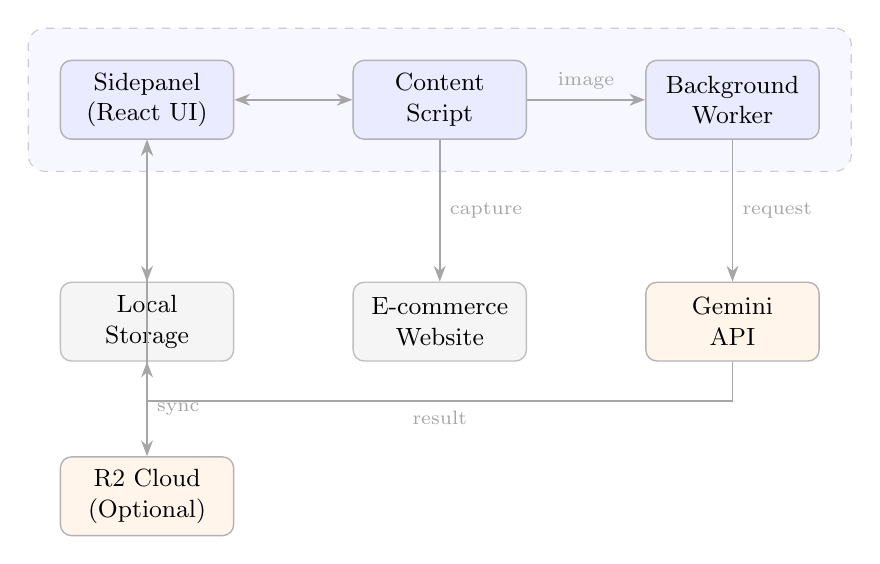
\begin{tikzpicture}[
    node distance=1.2cm and 1.5cm,
    % Extension components - subtle blue
    box/.style={
        rectangle, draw=gray!60, rounded corners=4pt,
        minimum width=2.2cm, minimum height=1cm,
        align=center, fill=blue!8, font=\small,
        line width=0.5pt
    },
    % External/browser components - light gray
    extbox/.style={
        rectangle, draw=gray!50, rounded corners=4pt,
        minimum width=2.2cm, minimum height=1cm,
        align=center, fill=gray!8, font=\small,
        line width=0.5pt
    },
    % Cloud services - subtle warm tone
    cloudbox/.style={
        rectangle, draw=gray!60, rounded corners=4pt,
        minimum width=2.2cm, minimum height=1cm,
        align=center, fill=orange!8, font=\small,
        line width=0.5pt
    },
    arrow/.style={-{Stealth[length=2mm, width=1.5mm]}, gray!70, line width=0.6pt},
    biarrow/.style={{Stealth[length=2mm, width=1.5mm]}-{Stealth[length=2mm, width=1.5mm]}, gray!70, line width=0.6pt},
    label/.style={font=\scriptsize, text=gray!70},
]

% Browser Extension Components - top row
\node[box] (sidepanel) {Sidepanel\\(React UI)};
\node[box, right=of sidepanel] (content) {Content\\Script};
\node[box, right=of content] (background) {Background\\Worker};

% Extension boundary
\begin{scope}[on background layer]
\node[draw=gray!40, dashed, rounded corners=6pt, fill=blue!3,
      fit=(sidepanel)(content)(background), inner sep=0.4cm,
      label={[anchor=south, font=\small\bfseries, text=gray!70]above:Browser Extension}] (extension) {};
\end{scope}

% External components - bottom row
\node[extbox, below=1.8cm of sidepanel] (storage) {Local\\Storage};
\node[extbox, below=1.8cm of content] (ecommerce) {E-commerce\\Website};
\node[cloudbox, below=1.8cm of background] (gemini) {Gemini\\API};

% Cloud storage - below local storage
\node[cloudbox, below=1.2cm of storage] (r2) {R2 Cloud\\(Optional)};

% Arrows with cleaner routing
\draw[biarrow] (sidepanel) -- (content);
\draw[arrow] (content) -- (background) node[midway, above, label] {image};
\draw[arrow] (content) -- (ecommerce) node[midway, right, label] {capture};
\draw[arrow] (background) -- (gemini) node[midway, right, label] {request};
\draw[biarrow] (sidepanel) -- (storage);
\draw[biarrow] (storage) -- (r2) node[midway, right, label] {sync};

% Result arrow - cleaner L-shaped path
\draw[arrow] (gemini.south) -- ++(0,-0.5) -| node[pos=0.25, below, label] {result} (sidepanel.south);

\end{tikzpicture}%
}
\caption{System architecture showing the interaction between browser extension components and cloud services.}
\label{fig:architecture}
\end{figure}

\subsection{User Photo Management}

The system implements a multi-layer storage strategy for user photographs:

\textbf{Local Storage Layer:} User images are stored in the browser's chrome.storage API as base64-encoded data URLs. This provides immediate access without network latency and ensures functionality even when offline.

\textbf{IndexedDB Layer:} For users who upload multiple photographs, images are stored in IndexedDB using the Dexie.js library, allowing efficient management of binary data with metadata such as timestamps and user-assigned names.

\textbf{Cloud Storage Layer (Optional):} Users can optionally configure Cloudflare R2 storage for cross-device synchronization. A lightweight Cloudflare Worker provides REST API endpoints for uploading, retrieving, and listing images. This enables users to access their photos and try-on history across multiple browsers and devices.

\subsection{Garment Image Capture}

A key innovation of our system is the intelligent capture of garment images from e-commerce websites. We implement two complementary capture methods:

\textbf{Context Menu Capture:} Users can right-click on any product image and select ``Try on this item'' from the context menu. The background service worker fetches the image, handles CORS restrictions through various fallback strategies, and converts the image to a base64 data URL for processing.

\textbf{Automatic Detection Mode:} When enabled, the content script monitors user clicks on the webpage. Upon detecting a click on a product image, the system employs an intelligent detection algorithm:

\begin{enumerate}
    \item Identify the clicked image element
    \item Check for modal overlays (common in e-commerce sites for enlarged product views) by scanning for elements with high z-index values
    \item If a modal is detected, find the largest image within it (typically the enlarged product view)
    \item If no modal exists, use the original clicked image
    \item Apply size filtering (minimum 150$\times$150 pixels) to exclude thumbnails and icons
    \item Convert the selected image to base64 format
\end{enumerate}

This automatic detection addresses a common e-commerce UX pattern where clicking a thumbnail opens a larger modal view. By detecting and capturing the enlarged image, we ensure higher quality inputs for the try-on generation.

Algorithm \ref{alg:autodetect} describes the automatic image detection process.

\begin{figure}[htbp]
\begin{algorithmic}[1]
\STATE \textbf{Input:} Click event on webpage
\STATE \textbf{Output:} Captured garment image (base64)
\STATE
\STATE clickedImg $\gets$ findImageAtClick(event)
\IF{clickedImg is null}
    \RETURN null
\ENDIF
\STATE
\STATE // Check for modal overlay
\STATE modalImages $\gets$ findImagesWithHighZIndex()
\IF{modalImages is not empty}
    \STATE selectedImg $\gets$ findLargestImage(modalImages)
\ELSE
    \STATE selectedImg $\gets$ clickedImg
\ENDIF
\STATE
\STATE // Validate size
\IF{selectedImg.width $<$ 150 OR selectedImg.height $<$ 150}
    \RETURN null
\ENDIF
\STATE
\STATE base64 $\gets$ convertToBase64(selectedImg)
\RETURN base64
\end{algorithmic}
\caption{Automatic garment image detection algorithm}
\label{alg:autodetect}
\end{figure}

\subsection{Try-On Generation Pipeline}

The core try-on generation leverages Google's Gemini multimodal models through their generative AI API. We utilize two model variants:

\begin{itemize}
    \item \textbf{Gemini 2.0 Flash (Image Generation):} Optimized for speed, providing results in approximately 15-20 seconds. Suitable for quick previews.

    \item \textbf{Gemini 3 Pro (Image Preview):} Higher quality generation with advanced reasoning capabilities, taking approximately 20-30 seconds. Recommended for final visualization before purchase decisions.
\end{itemize}

The generation process follows these steps:

\begin{enumerate}
    \item Parse user and garment images from data URLs to extract base64 content and MIME types
    \item Construct a carefully engineered prompt instructing the model to generate a single photorealistic try-on image
    \item Send the multimodal request containing the prompt and both images to the Gemini API
    \item Extract the generated image from the response
    \item Store the result in the history database and optionally sync to cloud storage
\end{enumerate}

The prompt engineering is critical for consistent results. Our prompt explicitly instructs the model to:
\begin{itemize}
    \item Generate exactly one output image (avoiding side-by-side comparisons)
    \item Preserve the person's face, body shape, pose, and background
    \item Only modify the clothing region
    \item Maintain realistic lighting and shadows
\end{itemize}

\subsection{Cross-Origin Resource Handling}

E-commerce websites often serve images from CDN domains different from the main website, creating CORS (Cross-Origin Resource Sharing) challenges. Our system implements multiple fallback strategies:

\begin{enumerate}
    \item \textbf{Canvas Method:} For same-origin or CORS-enabled images, we draw the image to a canvas element and export as data URL.

    \item \textbf{Fetch with Credentials:} Attempt to fetch the image with credentials included, which works for some CDN configurations.

    \item \textbf{Background Worker Fetch:} The service worker can fetch images without CORS restrictions that apply to content scripts.

    \item \textbf{Format Normalization:} Convert non-standard formats (WebP, GIF) to PNG through canvas rendering for consistent API input.
\end{enumerate}

\section{Implementation Details}

This section provides technical details of the implementation, including the technology stack, key components, and deployment considerations.

\subsection{Technology Stack}

The browser extension is built using modern web technologies:

\begin{itemize}
    \item \textbf{Extension Framework:} WXT (Web Extension Tools) 0.20 with Manifest V3 support for Chrome and Firefox compatibility
    \item \textbf{UI Framework:} React 19 with TypeScript for type-safe component development
    \item \textbf{State Management:} Zustand 5.0 with chrome.storage persistence middleware
    \item \textbf{Local Database:} Dexie.js 4.2 wrapping IndexedDB for efficient binary storage
    \item \textbf{Styling:} Tailwind CSS 4.1 with shadcn/ui components for consistent design
    \item \textbf{Cloud Worker:} Cloudflare Workers with R2 storage binding
    \item \textbf{AI Integration:} Google Generative AI SDK (@google/generative-ai)
\end{itemize}

\subsection{Extension Structure}

The extension follows a modular architecture with clear separation of concerns:

\textbf{Entrypoints:}
\begin{itemize}
    \item \texttt{sidepanel/} - Main user interface for photo management and try-on initiation
    \item \texttt{content.ts} - Content script for webpage interaction
    \item \texttt{content/autoMode.ts} - Automatic image detection logic
    \item \texttt{background.ts} - Service worker for API calls and messaging
    \item \texttt{result-popup/} - Standalone window for displaying try-on results
\end{itemize}

\textbf{Libraries:}
\begin{itemize}
    \item \texttt{lib/api/gemini.ts} - Gemini API integration with error handling and logging
    \item \texttt{lib/store/} - Zustand stores for application state
    \item \texttt{lib/storage/r2Storage.ts} - Cloudflare R2 operations
    \item \texttt{lib/db/index.ts} - IndexedDB schema and operations
\end{itemize}

\subsection{User Interface}

The side panel interface provides a streamlined workflow:

\begin{enumerate}
    \item \textbf{Photo Upload:} Users upload their photograph through drag-and-drop or file selection. The image is displayed as a preview and stored locally.

    \item \textbf{Garment Display:} When a garment image is captured (via right-click or auto-mode), it appears in the interface alongside the user photo.

    \item \textbf{Generation Controls:} A ``Try On'' button initiates generation, with a loading indicator showing progress. Users can select between fast and high-quality models.

    \item \textbf{Result Display:} Generated images appear in the interface with options to download, regenerate with different settings, or save to history.

    \item \textbf{History Gallery:} Previous try-on results are accessible in a gallery view, with options to favorite, delete, or view full-size images.
\end{itemize}

Figure \ref{fig:ui_sidepanel} shows the main user interface integrated with the Myntra e-commerce website.

\begin{figure}[htbp]
\centerline{\includegraphics[width=0.48\textwidth]{sidepanel.png}}
\caption{The browser extension sidepanel (right) integrated with the Myntra e-commerce website. The sidepanel displays the user's uploaded photo, a captured clothing item, and generation controls. Users can browse products while the extension remains accessible.}
\label{fig:ui_sidepanel}
\end{figure}

\subsection{Auto-Mode Implementation}

The automatic detection mode is implemented as a content script that attaches click listeners to the document. Key implementation details include:

\textbf{Debouncing:} A 3-second cooldown prevents rapid repeated captures when users click multiple times.

\textbf{Modal Detection:} The script scans for elements with z-index greater than 1000 (typical for modal overlays) and searches within them for image elements.

\textbf{Size Validation:} Images smaller than 150$\times$150 pixels are rejected to avoid capturing icons, logos, or thumbnail previews.

\textbf{Result Popup:} When auto-mode captures an image and generates a result, it opens in a separate popup window, allowing users to continue browsing while viewing the try-on result.

Figures \ref{fig:auto_mode_1} and \ref{fig:auto_mode_2} illustrate the auto-mode workflow.

\begin{figure}[htbp]
\centerline{\includegraphics[width=0.48\textwidth]{auto_mode_1.png}}
\caption{Auto-mode step 1: User browses a product page on Myntra. When the user clicks on the product image, the system prepares to capture it.}
\label{fig:auto_mode_1}
\end{figure}

\begin{figure}[htbp]
\centerline{\includegraphics[width=0.48\textwidth]{auto_mode_2.png}}
\caption{Auto-mode step 2: The modal with enlarged product image opens. The system automatically detects and captures the high-resolution image, triggering the generation process. A loading popup indicates that the try-on preview is being generated.}
\label{fig:auto_mode_2}
\end{figure}

\subsection{API Integration and Logging}

All API calls to the Gemini service are logged to IndexedDB for debugging and analytics purposes. Each log entry includes:

\begin{itemize}
    \item Timestamp and request type
    \item Model name and parameters
    \item Request/response sizes
    \item Duration in milliseconds
    \item Error details (if applicable)
\end{itemize}

This logging enables users to view their API usage history in the settings panel and helps diagnose issues when generation fails.

\subsection{Cloud Storage Architecture}

The optional Cloudflare R2 integration is implemented through a lightweight Worker that exposes REST endpoints:

\begin{itemize}
    \item \texttt{POST /upload} - Upload images with type classification (user, clothing, result)
    \item \texttt{GET /images/:key} - Retrieve images by key
    \item \texttt{DELETE /images/:key} - Delete images
    \item \texttt{GET /list/:type} - List images by type for gallery sync
    \item \texttt{GET /health} - Health check for connectivity testing
\end{itemize}

Images are stored with a key format of \texttt{\{type\}/\{timestamp\}-\{random\}}, ensuring uniqueness and enabling efficient listing by category. CORS headers allow access from the browser extension, and cache headers enable CDN caching for frequently accessed images.

\section{Evaluation and Comparison}

This section presents an evaluation of our system and compares it with existing virtual try-on approaches.

\subsection{Functional Evaluation}

We tested the system on the Myntra e-commerce platform, one of India's largest fashion retailers. The system successfully:

\begin{itemize}
    \item Captured product images from various page layouts including grid views and product detail pages
    \item Detected enlarged modal images when users clicked on thumbnails
    \item Generated try-on results across different garment categories including tops, dresses, and full outfits
    \item Preserved user identity features (face, body shape, pose) in generated images
\end{itemize}

Preliminary user testing with 2-3 participants indicated that users found the system convenient and easy to use. Participants appreciated the ability to try on clothes directly while browsing, without leaving the shopping website. Some challenges were identified with modal image detection on certain page layouts, which is an area for future improvement.

\subsection{Performance Characteristics}

Table \ref{tab:performance} summarizes the system's performance characteristics.

\begin{table}[htbp]
\caption{System Performance Characteristics}
\begin{center}
\begin{tabular}{|l|c|}
\hline
\textbf{Metric} & \textbf{Value} \\
\hline
Generation Time (Fast Model) & 15-20 seconds \\
\hline
Generation Time (Quality Model) & 20-30 seconds \\
\hline
Image Capture Time & $<$1 second \\
\hline
API Success Rate & $>$95\% \\
\hline
Modal Detection Rate & $\sim$70-90\% \\
\hline
Supported Garment Types & All categories \\
\hline
\end{tabular}
\label{tab:performance}
\end{center}
\end{table}

\subsection{Comparison with Existing Approaches}

Table \ref{tab:comparison} compares our approach with existing virtual try-on methods across several dimensions relevant to practical deployment.

\begin{table*}[htbp]
\caption{Comparison of Virtual Try-On Approaches}
\begin{center}
\begin{tabular}{|l|c|c|c|c|c|}
\hline
\textbf{Approach} & \textbf{GPU Required} & \textbf{Preprocessing} & \textbf{Platform} & \textbf{Auto-Capture} & \textbf{Accessibility} \\
\hline
VITON-HD \cite{vitonhd2021} & Yes (16GB+) & Parsing + Pose & Standalone & No & Research only \\
\hline
OOTDiffusion \cite{ootdiffusion2024} & Yes (16GB+) & Minimal & Standalone & No & Open source \\
\hline
IDM-VTON \cite{idmvton2024} & Yes (16GB+) & Minimal & Standalone & No & Open source \\
\hline
TryOnDiffusion \cite{tryondiffusion2023} & N/A & N/A & Proprietary & No & Not available \\
\hline
Commercial Tools & Cloud & Varies & Web app & No & Retailer integration \\
\hline
\textbf{Our Approach} & \textbf{No (Cloud API)} & \textbf{None} & \textbf{Browser ext.} & \textbf{Yes} & \textbf{Universal} \\
\hline
\end{tabular}
\label{tab:comparison}
\end{center}
\end{table*}

Key differentiators of our approach include:

\begin{enumerate}
    \item \textbf{No Local GPU:} By leveraging cloud APIs, users can generate try-on images on any device without requiring expensive GPU hardware.

    \item \textbf{No Preprocessing:} The multimodal LLM handles image understanding end-to-end, eliminating the need for separate human parsing or pose estimation models.

    \item \textbf{Universal Platform Support:} The browser extension works on any e-commerce website without requiring retailer cooperation or integration.

    \item \textbf{Automatic Image Capture:} The intelligent detection system captures product images automatically, reducing user friction.

    \item \textbf{Consumer Accessibility:} Unlike research tools that require technical expertise, our system can be used by everyday consumers.
\end{enumerate}

\subsection{Try-On Results}

Figure \ref{fig:results} shows an example try-on result generated by our system. The user's original photograph shows them wearing a white turtleneck sweater. When combined with a brown suede jacket captured from Myntra, the system generates a photorealistic image of the user wearing the jacket while preserving their facial features, body pose, and background.

\begin{figure}[htbp]
\centering
\includegraphics[height=3.5cm]{original.jpg}\hfill
\includegraphics[height=3.5cm]{garment.png}\hfill
\includegraphics[height=3.5cm]{tryon-result-1770140340273.png}

\vspace{2pt}
\small (a) User photo \hfill (b) Garment \hfill (c) Result\hspace{0.5cm}
\caption{Virtual try-on example: (a) Original user photograph, (b) Brown suede jacket from Myntra, (c) Generated result preserving identity features.}
\label{fig:results}
\end{figure}

\section{Discussion}

\subsection{Advantages of the Browser Extension Approach}

The browser extension paradigm offers several advantages for virtual try-on deployment:

\textbf{Universal Compatibility:} Unlike solutions that require e-commerce platform integration, our approach works immediately on any website displaying product images. This removes adoption barriers for both consumers and retailers.

\textbf{User Control:} Users maintain control over their photographs, which are stored locally or in their own cloud storage rather than on third-party servers. This addresses privacy concerns that might otherwise limit adoption.

\textbf{Seamless Workflow:} By integrating directly into the browsing experience, users can try on clothes without context switching to a separate application, maintaining their shopping flow.

\textbf{Zero Infrastructure for Users:} The cloud API approach means users do not need to install any software dependencies or have specific hardware requirements beyond a modern web browser.

\subsection{Potential Impact on E-commerce}

Virtual try-on technology has significant potential to reduce return rates in online fashion retail. By allowing customers to visualize how garments will look on them before purchase, we can:

\begin{itemize}
    \item Reduce ``bracketing'' behavior where customers order multiple sizes
    \item Decrease sizing-related returns, which constitute a major portion of fashion returns
    \item Lower environmental impact from reduced shipping and processing of returns
    \item Improve customer confidence in purchase decisions
\end{itemize}

While comprehensive studies of return rate reduction would require large-scale deployment and analysis, the fundamental premise that better visualization leads to more informed decisions is well-supported by retail research.

\subsection{Limitations}

Our current implementation has several limitations:

\textbf{Modal Detection Reliability:} The automatic image detection works well on most e-commerce sites but may fail on pages with non-standard modal implementations. Approximately 10-30\% of captures may require retry on certain sites.

\textbf{API Dependency:} The system relies on Google's Gemini API, introducing a dependency on external service availability and pricing. API rate limits may affect heavy users.

\textbf{Generation Quality Variability:} While the Gemini models generally produce good results, output quality can vary depending on input image quality, lighting conditions, and garment complexity.

\textbf{Limited Testing Scope:} Current testing has focused primarily on Indian e-commerce platforms (Myntra). Broader testing across international platforms (Amazon, ASOS, Zara) would strengthen validation.

\textbf{No Quantitative Evaluation:} We have not conducted formal user studies or quantitative comparisons with baseline methods, which would be valuable for demonstrating effectiveness.

\subsection{Future Work}

Several directions for future development are planned:

\begin{enumerate}
    \item \textbf{Improved Modal Detection:} Enhanced heuristics for detecting enlarged product images across diverse e-commerce layouts, potentially using machine learning for more robust detection.

    \item \textbf{Multi-Garment Try-On:} Support for trying on complete outfits by combining multiple garment items in a single generation.

    \item \textbf{Size Recommendation:} Integration with sizing APIs to provide size recommendations alongside visual try-on.

    \item \textbf{Video Try-On:} Extension to short video clips showing the garment from multiple angles or with movement.

    \item \textbf{Offline Support:} Exploration of on-device models for try-on generation without API dependency, as edge AI capabilities improve.

    \item \textbf{Retailer Analytics:} Optional anonymized analytics for retailers to understand which products are being tried on, potentially informing inventory decisions.
\end{enumerate}

\section{Conclusion}

This paper presented a novel approach to virtual try-on technology through a browser extension that integrates seamlessly with existing e-commerce platforms. By leveraging multimodal large language models through cloud APIs, our system eliminates the infrastructure barriers that have limited practical deployment of virtual try-on technology.

The key contributions include: (1) a browser extension architecture that works universally across e-commerce websites without retailer integration; (2) an intelligent automatic image detection system that captures product images with minimal user effort; (3) integration with state-of-the-art multimodal AI through cloud APIs, removing local GPU requirements; and (4) a multi-layer storage architecture supporting both local and cloud-synchronized operation.

While challenges remain in detection reliability and API dependency, the system demonstrates that practical, accessible virtual try-on is achievable with current technology. As multimodal AI capabilities continue to advance and become more accessible, we anticipate that virtual try-on will become a standard feature of online shopping, helping consumers make more informed decisions and reducing the economic and environmental costs of product returns.

The browser extension approach represents a path toward democratizing virtual try-on technology, making it available to any consumer shopping on any e-commerce platform, rather than limiting it to retailers who have invested in custom integrations.

\section*{Acknowledgment}

We thank Google for providing access to the Gemini API through their generative AI platform, and Cloudflare for their R2 storage service that enables the cloud synchronization features of this system.

\begin{thebibliography}{00}

\bibitem{viton2018}
X. Han, Z. Wu, Z. Wu, R. Yu, and L. S. Davis, ``VITON: An Image-based Virtual Try-on Network,'' in \textit{Proceedings of the IEEE Conference on Computer Vision and Pattern Recognition (CVPR)}, 2018, pp. 7543-7552.

\bibitem{vitonhd2021}
S. Choi, S. Park, M. Lee, and J. Choo, ``VITON-HD: High-Resolution Virtual Try-On via Misalignment-Aware Normalization,'' in \textit{Proceedings of the IEEE/CVF Conference on Computer Vision and Pattern Recognition (CVPR)}, 2021, pp. 14131-14140.

\bibitem{tryondiffusion2023}
L. Zhu, D. Yang, T. Zhu, F. Reda, W. Chan, C. Saharia, M. Norouzi, and I. Kemelmacher-Shlizerman, ``TryOnDiffusion: A Tale of Two UNets,'' in \textit{Proceedings of the IEEE/CVF Conference on Computer Vision and Pattern Recognition (CVPR)}, 2023, pp. 4606-4615.

\bibitem{ootdiffusion2024}
Y. Xu, T. Gu, W. Chen, and C. Chen, ``OOTDiffusion: Outfitting Fusion based Latent Diffusion for Controllable Virtual Try-on,'' in \textit{Proceedings of the AAAI Conference on Artificial Intelligence}, vol. 39, no. 9, 2025, pp. 8996-9004.

\bibitem{idmvton2024}
Y. Choi, S. Kwak, K. Lee, H. Choi, and J. Shin, ``IDM-VTON: Improving Diffusion Models for Authentic Virtual Try-on in the Wild,'' in \textit{Proceedings of the European Conference on Computer Vision (ECCV)}, 2024.

\bibitem{ldm2022}
R. Rombach, A. Blattmann, D. Lorenz, P. Esser, and B. Ommer, ``High-Resolution Image Synthesis with Latent Diffusion Models,'' in \textit{Proceedings of the IEEE/CVF Conference on Computer Vision and Pattern Recognition (CVPR)}, 2022, pp. 10684-10695.

\bibitem{ddpm2020}
J. Ho, A. Jain, and P. Abbeel, ``Denoising Diffusion Probabilistic Models,'' in \textit{Advances in Neural Information Processing Systems (NeurIPS)}, vol. 33, 2020, pp. 6840-6851.

\bibitem{densepose2018}
R. A. G{\"u}ler, N. Neverova, and I. Kokkinos, ``DensePose: Dense Human Pose Estimation in the Wild,'' in \textit{Proceedings of the IEEE Conference on Computer Vision and Pattern Recognition (CVPR)}, 2018, pp. 7297-7306.

\bibitem{nrf2024}
National Retail Federation and Happy Returns, ``2024 Consumer Returns in the Retail Industry,'' NRF Report, 2024. [Online]. Available: https://nrf.com/research/2024-consumer-returns-retail-industry

\bibitem{coresight2023}
Coresight Research, ``US Online Apparel Return Rates and the Impact on Retailers,'' Coresight Research Report, 2023.

\bibitem{stableviton2024}
J. Kim, S. Gu, G. Park, S. Park, S. Choi, and J. Choo, ``StableVITON: Learning Semantic Correspondence with Latent Diffusion Model for Virtual Try-On,'' in \textit{Proceedings of the IEEE/CVF Conference on Computer Vision and Pattern Recognition (CVPR)}, 2024.

\bibitem{dresscode2022}
D. Morelli, M. Fincato, M. Cornia, F. Landi, F. Cesari, and R. Cucchiara, ``Dress Code: High-Resolution Multi-Category Virtual Try-On,'' in \textit{Proceedings of the IEEE/CVF Conference on Computer Vision and Pattern Recognition (CVPR)}, 2022.

\bibitem{ladivton2023}
D. Morelli, A. Baldrati, G. Cartella, M. Cornia, M. Bertini, and R. Cucchiara, ``LaDI-VTON: Latent Diffusion Textual-Inversion Enhanced Virtual Try-On,'' in \textit{Proceedings of the ACM International Conference on Multimedia (MM)}, 2023.

\bibitem{gpvton2023}
P. Xie, X. Huang, X. Hu, Z. Li, K. Zheng, and M. Lyu, ``GP-VTON: Towards General Purpose Virtual Try-on via Collaborative Local-Flow Global-Parsing Learning,'' in \textit{Proceedings of the IEEE/CVF Conference on Computer Vision and Pattern Recognition (CVPR)}, 2023.

\bibitem{hrviton2022}
S. Lee, G. Gu, S. Park, S. Choi, and J. Choo, ``High-Resolution Virtual Try-On with Misalignment and Occlusion-Handled Conditions,'' in \textit{Proceedings of the European Conference on Computer Vision (ECCV)}, 2022.

\bibitem{clip2021}
A. Radford, J. W. Kim, C. Hallacy, A. Ramesh, G. Goh, S. Agarwal, G. Sastry, A. Askell, P. Mishkin, J. Clark, G. Krueger, and I. Sutskever, ``Learning Transferable Visual Models From Natural Language Supervision,'' in \textit{Proceedings of the International Conference on Machine Learning (ICML)}, 2021, pp. 8748-8763.

\bibitem{ipadapter2023}
H. Ye, J. Zhang, S. Liu, X. Han, and W. Yang, ``IP-Adapter: Text Compatible Image Prompt Adapter for Text-to-Image Diffusion Models,'' \textit{arXiv preprint arXiv:2308.06721}, 2023.

\bibitem{deepfashion2016}
Z. Liu, P. Luo, S. Qiu, X. Wang, and X. Tang, ``DeepFashion: Powering Robust Clothes Recognition and Retrieval with Rich Annotations,'' in \textit{Proceedings of the IEEE Conference on Computer Vision and Pattern Recognition (CVPR)}, 2016, pp. 1096-1104.

\bibitem{schp2020}
K. Li, S. He, B. Feng, S. Wu, S. Liu, J. Shao, and K. Li, ``Self-Correction for Human Parsing,'' \textit{IEEE Transactions on Pattern Analysis and Machine Intelligence}, vol. 44, no. 6, pp. 3260-3271, 2022.

\end{thebibliography}

\end{document}
